% =============================================================================
% Working extract -- Results, Q1 section only.
% Extracted from documentation/refocus_draft/20th_1_31_pm_audited.tex on 2026-08-21.
% Content fragment, NOT a standalone compilable document -- equations/labels it
% references (e.g. eq:mean-cr-residual, eq:cr) are defined in that file's
% Methodology chapter, not here.
% Purpose: isolated iteration on this Q's Results section (claim verification +
% rewrites) without touching the shared main file. Merge back into
% 20th_1_31_pm_audited.tex once settled -- do not edit the main file's copy of
% this section while this working copy is in progress, to avoid divergence.
% =============================================================================

\section{Q1: What explains a plot's persistent departure from the shared curve?}

Using the 4-survey cohort, canopy cover and thinning history dominate the attribution in every feature set and every method tested (Table~\ref{tab:results-q1}).

\begin{table}[!htbp]
\centering
\scriptsize
\renewcommand{\arraystretch}{1.2}
\begin{tabular}{lrlll}
\toprule
Set & n rows & EN R2 [95\% CI] & XGB R2 [95\% CI] & LMM spatial variance explained \\
\midrule
Set1 (baseline only) & 71{,}766 & 0.220 [0.180, 0.252] & 0.222 [0.183, 0.252] & 0.016$\pm$0.078 \\
Set2 & 71{,}766 & 0.359 [0.310, 0.396] & 0.416 [0.355, 0.461] & 0.204$\pm$0.066 \\
Set3 & 71{,}727 & 0.325 [0.272, 0.365] & 0.375 [0.321, 0.414] & 0.049$\pm$0.048 \\
Set4 & 71{,}330 & 0.358 [0.305, 0.398] & 0.395 [0.338, 0.438] & 0.175$\pm$0.064 \\
\bottomrule
\end{tabular}
\caption{\small{Attribution of the persistent mean curve residual (Equation~\ref{eq:mean-cr-residual}),
4survey only, spatial-block split.}}
\label{tab:results-q1}
\end{table}

These $R^2$ values are modest in absolute terms: even the best set (Set2, XGBoost, $R^2=0.416$) leaves more than half the variation in a plot's persistent curve departure unexplained by the tested environmental and management features. The value of these models lies in identifying which conditions are associated with departures, not in precisely predicting how large a given plot's departure will be. $R^2$ is not directly comparable between Q1 and Q2, or between Q1/Q2 and Q3: each predicts a different target with different underlying variance, so a higher or lower number in one section does not by itself mean a stronger or weaker model.

% AUDIT: the table above reports only pooled R2/CI and LMM variance-explained. The coefficient values, SHAP ranks, VIF, ICC and within-compartment correlation numbers that carry the actual argument below appear nowhere in a table or figure -- currently text-only. The commented-out \fig{} composite sketch further below already scopes the fix (coefficient forest plot + Moran's I by set + residual map); building it would let a good share of the numeric prose below shorten in favour of "see Figure X."
\subsection{Discussion}
\textbf{Canopy cover and thinning history dominate the attribution in every feature set and both methods -- but because canopy cover comes from the same LiDAR pipeline as the height targets, this could just be the target restated in different units.} Canopy cover carries the largest or near-largest Elastic Net coefficient in every set (Set4: +1.943$\pm$0.034), and ranks first by mean $|$SHAP$|$ in every XGBoost set (1.375--1.442).

This raises an obvious concern: canopy cover is measured from the same LiDAR survey as the height target itself, so a large coefficient could just mean the model has found a disguised copy of the target, not a real driver. Three checks test this directly. First, canopy cover's correlation with all three of this project's targets is moderate (Pearson 0.35--0.47), not near 1 -- it is not simply the target restated in different units. Second, removing canopy cover from Set4 and refitting drops $R^2$ by roughly a third for both models (Elastic Net: 0.350 to 0.231; XGBoost: 0.388 to 0.249) -- a bigger drop than its SHAP margin alone (1.2--1.7$\times$ the next variable) would suggest, meaning it carries signal nothing else in the set backfills. Third, the variable most likely to absorb that gap, $\mathit{dist}_{\text{to\_road}}$, does not: its own SHAP value moves slightly the wrong way (1.003 to 0.869). Together, these rule out simple correlation-driven credit transfer as the mechanism, though they do not explain why canopy cover carries this much unique signal in the first place.

The defensible reading: treat canopy cover and thinning as baseline stand-structure controls, expected to dominate by construction. The actual attribution question is what the true environmental variables contribute beyond that baseline.

%TODO: DEFINE ABIOTIC IN THE INTRO OR RELATED WORK.
\textbf{Among abiotic (non-biological, environmental) predictors, only slope is stable across methods; topex (a wind-exposure measure) splits the two models -- a genuine disagreement, not a shared signal.}
Among abiotic predictors, only $\mathit{slope\_degrees}$ was stable across both methods, showing consistent positive effects in LMM (+0.894/+0.861) and Elastic Net (+1.230/+0.993) across Sets~3 and 4. In contrast, $\mathit{topex}$ revealed a clear split: LMM found a strong, stable positive link (+1.316/+1.323), whereas Elastic Net yielded weak estimates that flipped signs ($-0.175$ in Set~3 to $+0.063$ in Set~4) with high variance. This reflects a genuine disagreement between models rather than a robust, shared signal. A few reasons below were explored: 

Two simpler explanations were checked and ruled out. Multicollinearity is not the cause: the unstable predictors ($\mathit{tas\_mean}$, $\mathit{soilgrids\_ph}$, $\mathit{topex}$; VIF 2.1--3.4) all have \emph{lower} collinearity than the stable $\mathit{chelsa\_bio12\_precip\_mm}$ (VIF 3.91). Climate-data timing is not the cause either: $\mathit{chelsa\_bio12\_precip\_mm}$ uses a static 1981--2010 climate normal and stays stable, while $\mathit{tas\_mean}$ uses year-matched data and is unstable -- the opposite of what a timing-mismatch explanation would predict, and it does not explain $\mathit{soilgrids\_ph}$ (a static soil trait) being unstable at all.
%TODO: add this static or changing through survey years in the data table.

A third possible reason is spatial confounding. Unlike LMM, Elastic Net does not group data by compartment. If a variable mainly changes from one compartment to the next, Elastic Net can easily confuse it with other unmeasured local factors. We checked this by measuring between-compartment variation (ICC). The unstable variables all scored high: $\mathit{topex}$ (0.74), $\mathit{soilgrids\_ph}$ (0.77), and $\mathit{tas\_mean}$ (0.89). However, the stable rainfall variable ($\mathit{chelsa\_bio12\_precip\_mm}$) scored even higher at 0.97. This shows that high spatial variation alone does not make a variable unstable; it makes confounding possible, but is not enough to cause it by itself.

%---
\textbf{One mechanism explains all three cases: whether a real local signal survives removing between-compartment differences.} % AUDIT: this account was built and tested on the same data that produced the instability finding it explains -- a plausible, evidenced mechanism, but not validated on an independent split. Read as the best-evidenced account so far, not a fully confirmed one.
Because both models assume linear relationships, raw non-linearity alone cannot be the cause; the key difference is LMM's compartment random intercept. Mean-centring variables and targets within each compartment isolates this local signal directly:

\begin{itemize}
    \item $\mathit{topex}$ shows a real local signal: its within-compartment correlation rises from 0.09 to 0.21 and becomes monotonic. LMM captures this local effect via random intercepts, whereas Elastic Net pools the data and confuses the signal.
    \item $\mathit{tas\_mean}$ and $\mathit{soilgrids\_ph}$ show almost no local signal: within-compartment correlations collapse from 0.27 to 0.08 and 0.05. Their raw correlations are between-compartment artifacts, leaving no real relationship to estimate reliably.
    \item $\mathit{chelsa\_bio12\_precip\_mm}$ maintains a clean, monotonic local link ($-0.11$ vs.\ $-0.36$ raw), which anchors a stable Elastic Net coefficient despite high spatial variance.
\end{itemize}

Apparent non-linearity in the pooled data is therefore a byproduct of spatial confounding. Variables with genuine local effects stay stable or resolve under random-intercept models, while those driven by between-compartment differences break down (see Appendix~\ref{app:nonlinearity-check}).
%---

\textbf{Both models leave significant spatial clustering in their residuals, but XGBoost removes far more of it than Elastic Net as environmental data is added.} All feature sets leave significant spatial autocorrelation in their residuals (distance-band Moran's $I$ at 1385--1739\,m, $p = 0.001$). The two models remove this clustering at very different rates: Elastic Net drops it by only 29\% (0.145 $\to$ 0.103), while XGBoost drops it by 63\% (0.146 $\to$ 0.054). % THEORY, UNTESTED: XGBoost's own flexibility (automatic non-linear interactions) plausibly explains this \cite{zou2005Regularization_C4_NN}, but the same flexibility could also just be fitting spatial noise -- not distinguished here.
Some clustering remains unmodelled in both cases, pointing to unmeasured environmental factors, resolution limits, or genuine spatially varying processes \cite{gaspard2019Residual_C5_EVAL}.

Set~3 (terrain-only) is the weakest feature set. A category-level refit on Set~4 shows soil adds only a small gain ($+0.022$ $R^2$), while climate actively \emph{reduces} accuracy ($-0.056$ $R^2$) -- terrain and spatial-edge-effect variables drive most of Set~4's advantage instead (full ablation in Appendix~\ref{app:category-ablation}). This runs against the general expectation that forest productivity depends on mixed biophysical inputs \cite{bontemps2014Predictive_C2_BG}; here, climate data adds instability rather than predictive value.

Every environmental set's $R^2$ confidence interval clears the baseline (Set~1) with no overlap -- real evidence that environmental features help at all. But XGBoost's own intervals for Set~2 and Set~4 overlap ([0.355, 0.461] vs.\ [0.338, 0.438]), so which of those two sets is actually better cannot be said with confidence.

% AUDIT: this file previously carried two near-duplicate "For Q1" synthesis paragraphs (a leftover from the multi-session file reorganisation); merged into one below, given its own subsection per the requested structure.

\begin{figure}[!htbp]
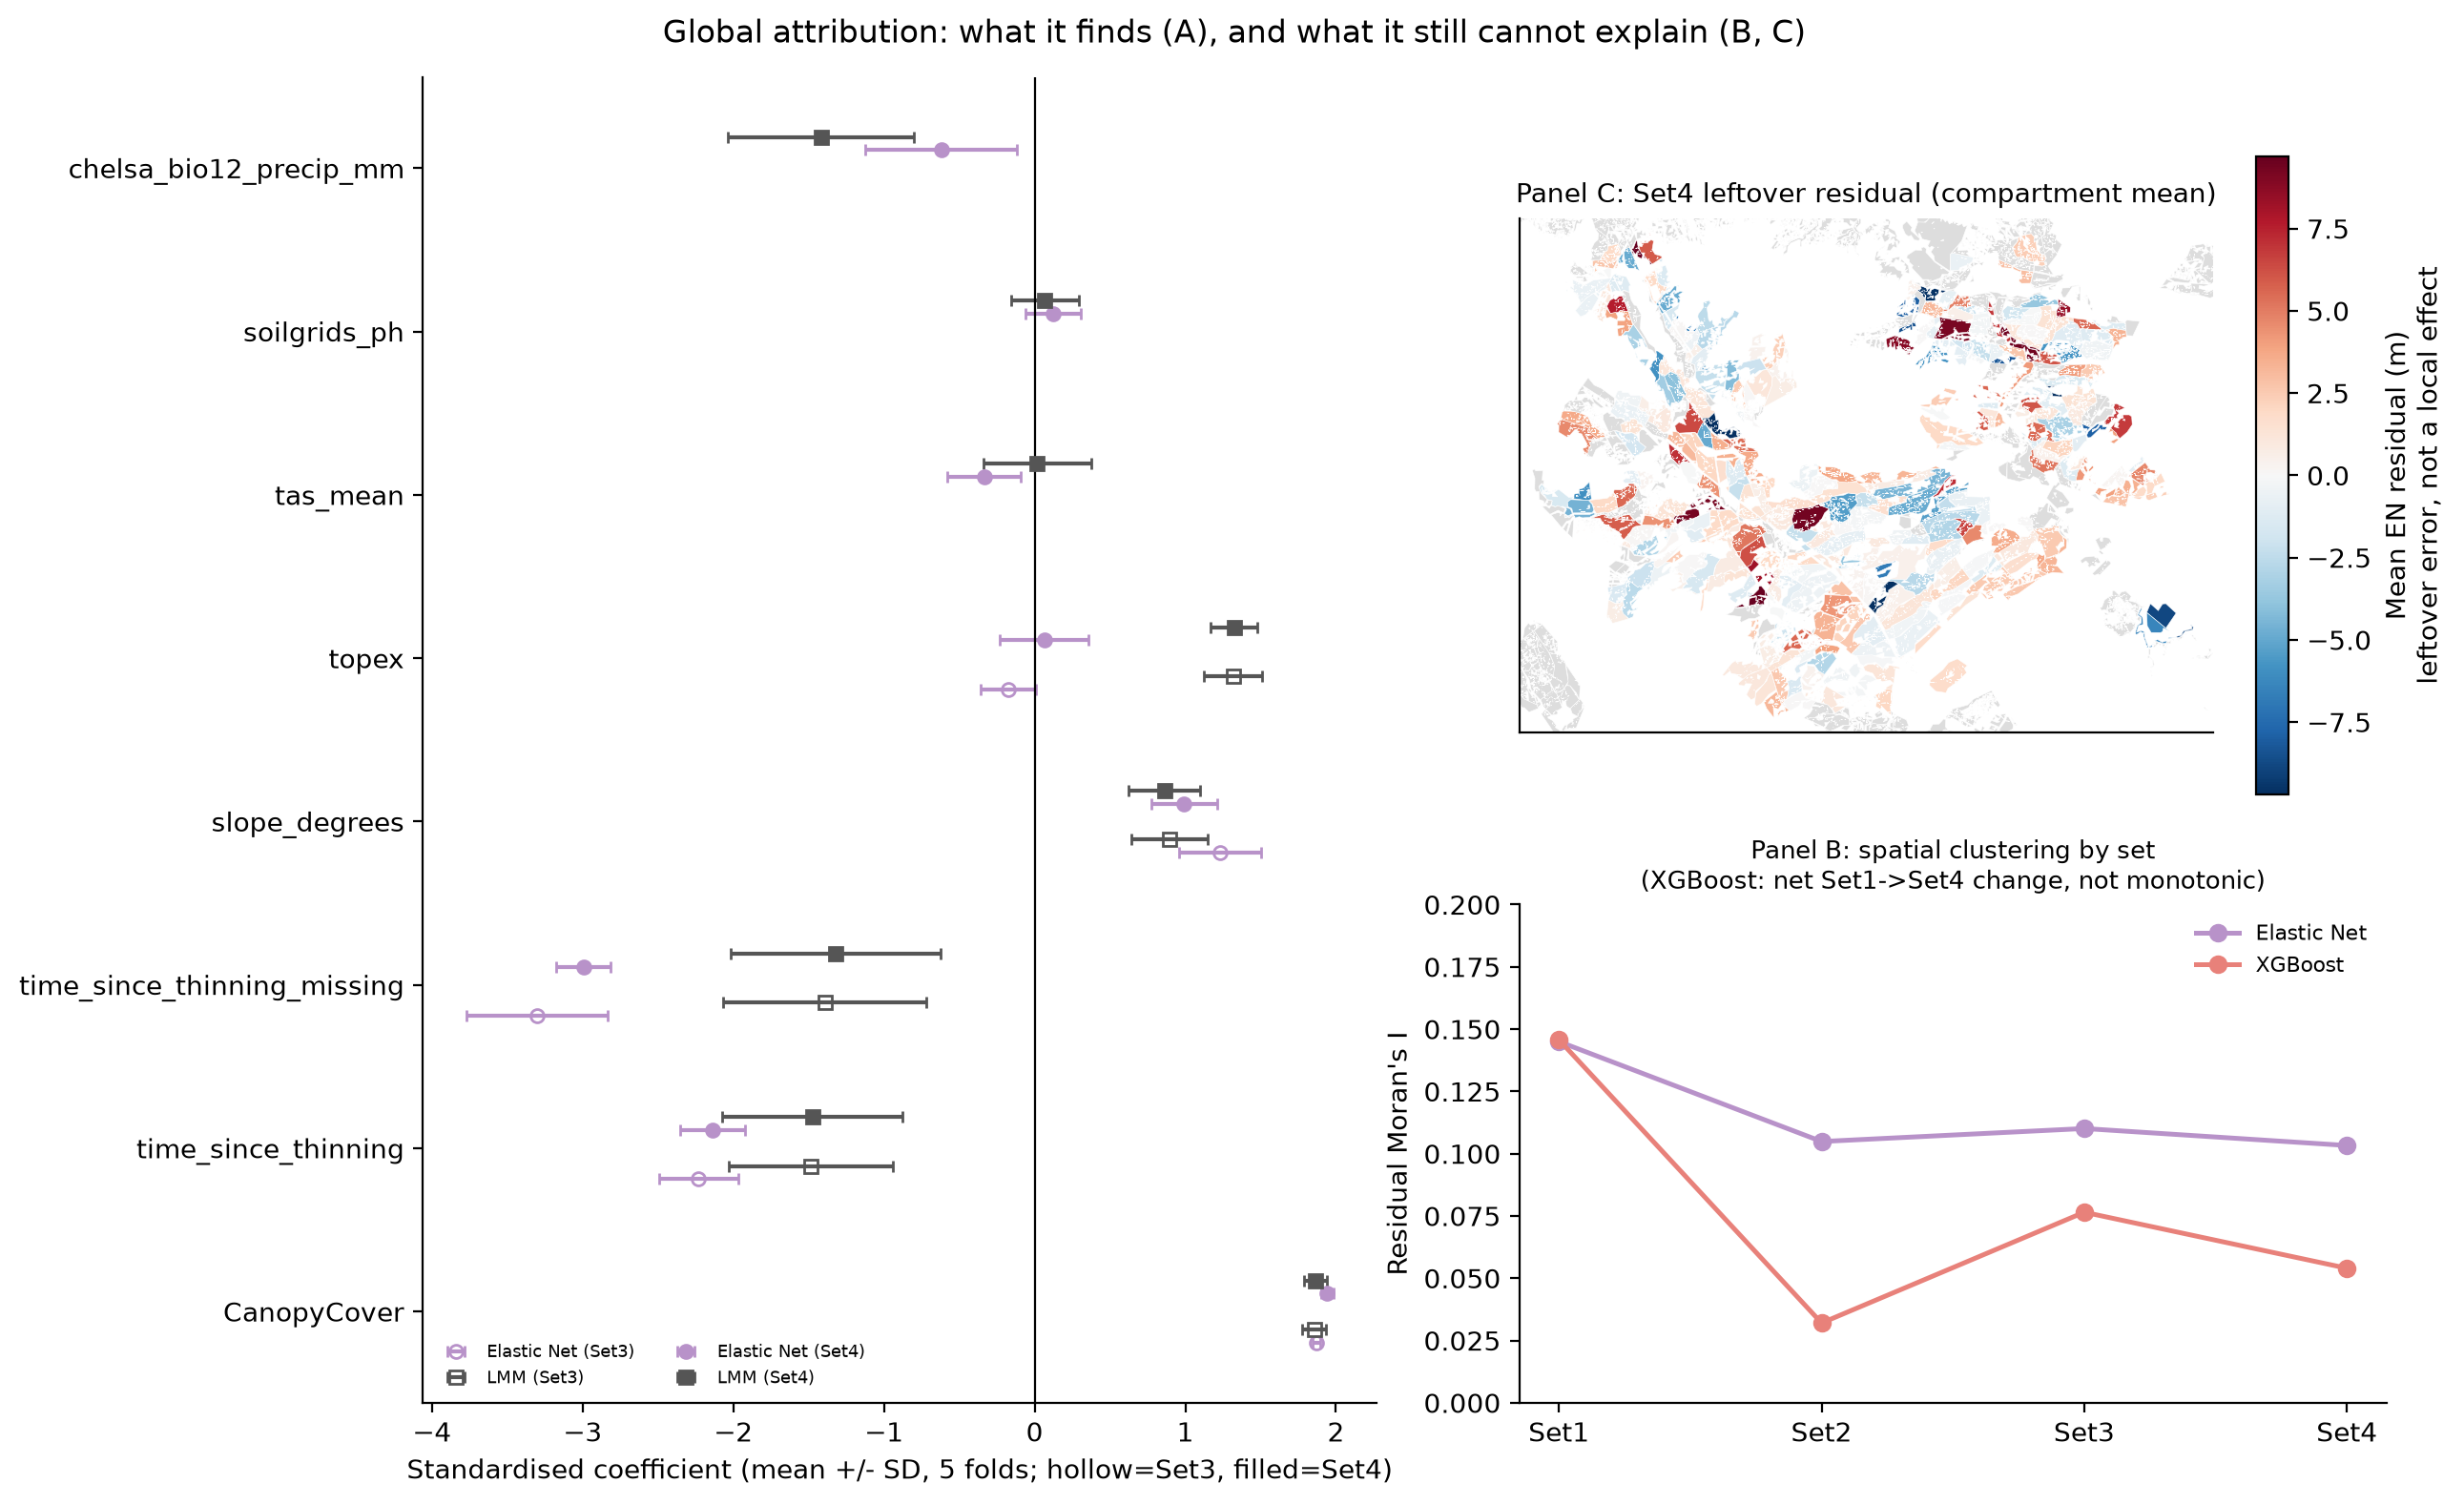
\includegraphics[width=\textwidth]{figures/fig_results/q1_attribution_composite.png}
\caption{% AUDIT: placeholder caption -- image file exists (built recently) but has not yet been described or interpreted in text. Needs: what each panel shows, and how it relates to the coefficient/VIF/ICC findings below (see the table-vs-discussion mismatch note above the results table).
--- headline result in caption form : then what each graph is and how to read it. }
\label{fig:q1-attribution-composite}
\end{figure}


% \fig{\textbf{Q1 -- coefficient/Moran's I/residual-map composite.} Three panels.
% Panel A (attribution): coefficient forest plot, one row per variable (\texttt{CanopyCover},
% both thinning columns, \texttt{slope\_degrees}, \texttt{topex}, the climate/soil
% variables), point = mean, whisker = fold SD, LMM and EN as two colours/markers side by
% side, Set3 and Set4 as two sub-columns -- the visual payoff of the slope-stable/
% topex-unstable contrast, otherwise the reader has to hold four numbers in their head.
% Panel B (spatial clustering responds unevenly to environmental data): Moran's I by set
% (Set1--Set4), EN and XGBoost as two lines -- EN nearly flat, XGBoost dropping
% substantially, the divergence between the two lines is the finding, not a shared trend.
% Panel C (where the leftover residual sits): a map of Set4/4survey's model residual,
% coloured by magnitude/sign -- this is what motivates Q2, earning its panel on
% structural grounds, not decoration. Establishes: none of this (coefficients, the
% Moran's I trend, the spatial residual pattern) exists in any table in this chapter, all
% of it is currently text-only. Answers Q1 items 1--3.}


%maybe when we comapre differencce ebtween 4 survey and 6 survey, we can say that as 6 survey is morehomogenous, we know it has a sifferent CR fit, then (((this oudlbe a reaosn or justifcation) for something)) 

\subsection*{Conclusion}
Stand structure and management account for most of a plot's deviation from the baseline curve; among abiotic variables, only slope is consistently stable across methods. Instability elsewhere depends on whether a genuine local signal survives between-compartment pooling: LMM recovers a real local relationship for topex that Elastic Net obscures, whereas tas\_mean and soilgrids\_ph are largely between-compartment artifacts. At the category level, soil adds a slight gain while climate harms performance. Significant spatial autocorrelation persists in both models' residuals (Moran's $I$ falls 29\% in EN vs.\ 63\% in XGBoost), so global environmental features do not capture all spatial structure -- directly motivating the spatially varying model tested in Q2.
